\section{Lab 2}
\label{sec:lab2}
For the second part of the lab the task is to parallelize a serial implementation of the Red-Back Gauss-Seidal algorithm. This is done using OpenMP (Open \textbf Multi-\textbf Processing) which is an API for forming multi-threaded programs in C, C++ and, Fortran. This parallel version is evaluated using the same simulator and CCP:s as in \nameref{sec:lab1}. 

\subsection{Task 1}
The program reads a matrix on the form $n \times n, n \in [4,8,25,100,200]$ containing data points from a file. To make the program simpler and avoid special cases a padding is added to the matrix changing its dimensions to $(n+2) \times (n+2)$. Then every other data point, here by called red dots, is looped through. For every red dot an average of itself and its neighbors to the west, south, north, and east is calculated and written as the dots new value. For all the other data points, called black dots, the same thing is performed. The difference of the dots new and old value is added together and the process is repeated until this accumulated difference of averages, divided by $n^2$, is smaller than $0.01$. After the program finishes its execution the matrix have converged to an average of all red and black dots.

The distribution of the red and black dots forms a chess pattern. This means that when we calculate the average for a dot and its neighbors, all the neighbors are of the other color. As such, when going through for example the red dots there is no need to invalidate any other dots because the black dots are only read and you are the only one accessing your red dot.

\subsection{Task 2}
In listing~\ref{lst:solve} a parallelized version of the function \texttt{void Solve(double **A)} are shown. The parallelization have been done using directives from the OpenMP API. Only this function is shown as the other parts of the program for reading the input file and printing to the console is not included in the performance analysis. The approach taken for making the function execute in parallel is to distribute the lines of the matrix evenly between all threads. This is done twice, once for the red dots and once for the black. Only one thread resets \texttt{diff} to zero on line 5 and test whether the program is finished or not on line 25. At each for loop that goes through the red and black dots the directive \texttt{reduction(+:diff)} is used which causes each thread to have its own private version of \texttt{diff} that all gets added together after the for loop.

\centerline{
\begin{minipage}{1.0\textwidth}
\lstinputlisting[caption={\textit{Parallel version of original} \texttt{void Solve(double **A).}}, label={lst:solve}]{include/solve.c}
\end{minipage}
}
\subsection{Task 3}
\todo[inline]{
Evaluate MSI, MESI, and MESI+migratory in the context of this benchmark. Perform a detailed characterization of the benchmark using different protocols. Discuss how the behavior changes when the working set size is modified. Show how execution time relates to the cache access statistics.}



Samma mönster som i Lab 1, MSI får mer writemiss osv än MESI vilket gör MESI lite bättre.
\begin{figure}[t]
	\center
	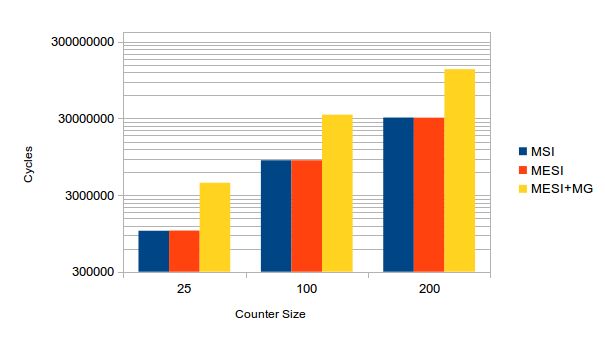
\includegraphics[width=0.8\textwidth]{lab2bars}
	\caption{Results from simulation of the parallelized benchmark for all cache coherence protocols combined with different working sets.}
	\label{fig:resultslab1}
\end{figure}

\subsection{Task 4}
\todo[inline]{
Outline a strategy to modify the MESI protocol to support the O state.
Analyze the MESI\_SMPCache.cpp source to understand how the MESI protocol is currently modeled.
Discuss changes that need to be made to the readLine, writeLine, readRemoteAction, and writeRemoteAction functions. Show the necessary changes in pseducode. Should the code that tracks cache access statistics be modified? If so, how?}